\documentclass[compress]{beamer}
%\documentclass[handout]{beamer}

\mode<presentation>
{
  \usetheme{CambridgeUS}      % or try Darmstadt, Madrid, Warsaw, ...
  \usecolortheme{default} % or try albatross, beaver, crane, ...
  \usefonttheme{default}  % or try serif, structurebold, ...
  \setbeamertemplate{navigation symbols}{}
  \mode<beamer>{\setbeamertemplate{blocks}[rounded][shadow=true]}
  \setbeamertemplate{caption}[numbered]
  \useoutertheme{infolines}
  \useoutertheme[subsection=false]{miniframes}
} 

\usepackage[english]{babel}
\usepackage[utf8x]{inputenc}
\usepackage{pifont}
\usepackage{amssymb}
\usepackage{xcolor}
\usepackage{tikz}
\newcommand{\xmark}{\ding{55}}%
\usepackage{eurosym}
\usepackage{graphicx}
% set colors
\definecolor{myNewColorA}{RGB}{0, 45,114}
\definecolor{myNewColorB}{RGB}{0, 45,114}
\definecolor{myNewColorC}{RGB}{0, 45,114} % {130,138,143}
\setbeamercolor*{palette primary}{bg=myNewColorC}
\setbeamercolor*{palette secondary}{bg=myNewColorB, fg = white}
\setbeamercolor*{palette tertiary}{bg=myNewColorA, fg = white}
\setbeamercolor*{titlelike}{fg=myNewColorA}
\setbeamercolor*{title}{bg=myNewColorA, fg = white}
\setbeamercolor*{item}{fg=myNewColorA}
\setbeamercolor*{caption name}{fg=myNewColorA}
\setbeamercolor{date in head/foot}{fg=white}
\setbeamercolor{page number in head/foot}{fg=white}


\titlegraphic{%
\vspace{0cm}
    
\includegraphics[width=4cm]{logo-vertical2.png}
}

\usepackage{subcaption}
% \usepackage{mathrsfs}

\usepackage{dirtytalk}
\usepackage{tcolorbox}
\usepackage{multicol}
\usepackage{multirow}
\usepackage{caption}
\usepackage{threeparttable}
\usepackage{pdfpages}
\usepackage{longtable}
\usepackage{adjustbox}
\usepackage{colortbl}
\usepackage{tikz}
\def\checkmark{\tikz\fill[scale=0.4](0,.35) -- (.25,0) -- (1,.7) -- (.25,.15) -- cycle;} 
\usepackage{pdfpages}

\usepackage{accents}
\newcommand{\ubar}[1]{\underaccent{\bar}{#1}}
%\usepackage{enumitem}

%% References - BEGIN
\usepackage[backend=bibtex8,style=authoryear-icomp,doi=false,url=false,isbn=false,eprint=false]{biblatex}
\renewbibmacro{in:}{}		% gets rid of the 'In' in front of the journal name
%\bibliographystyle{natbib}        
% \bibliography{references.bib}

% diagram (tree)
\usepackage{tikz}
\tikzset{
  treenode/.style = {shape=rectangle, rounded corners,
                     draw, align=center,
                     top color=white,
                     bottom color=blue!20},
  root/.style     = {treenode, font=\Large,
                     bottom color=red!30},
  env/.style      = {treenode, font=\ttfamily\normalsize},
  dummy/.style    = {circle,draw}
}

% Title page details: 
\title{Chapter 4: Supply and Demand} 
\author{Jamie Hyder \\
    Discussion section 4}
\date{September 12, 2023}

\begin{document}

% Title page
\begin{frame}
    \titlepage 
\end{frame}

% Outline frame
\begin{frame}{Outline}
    These slides will introduce the critical concepts of \textbf{\textit{supply}} and \textbf{\textit{demand}}:\textit{ the behavior of firms and individuals as they interact in competitive markets.}
    
    \medskip
    \medskip

    We will see how these two forces interact to determine prices.
\end{frame}

\begin{frame}{Features of a market}
    \begin{enumerate}
        \item What is a market?
        \item What are some examples of markets?
        \item What does it mean for a market to be \textit{competitive}?
        \item Are all markets competitive?
        \item What makes a market perfectly competitive?
    \end{enumerate}
\end{frame}

\begin{frame}{Perfectly competitive markets}
    In a perfectly competitive market:
    \begin{enumerate}
        \item The market is competitive: There are many buyers are sellers so that no individual has an impact on price
        \item All goods are identical
    \end{enumerate}
    \medskip
    \begin{center}
    A consequence of 1: All actors are \textit{price-takers}
    \end{center}
\end{frame}

% How people make decisions
\begin{frame}{Demand} 
\begin{itemize}
    \item     What is the \textit{quantity demanded} of a good?
    \item     What is the \textit{law of demand}?
    \item     What is the difference between a demand schedule and a demand curve?
\end{itemize}
\end{frame} 



\begin{frame}
    \frametitle{Demand schedule and curve}
    \centering
    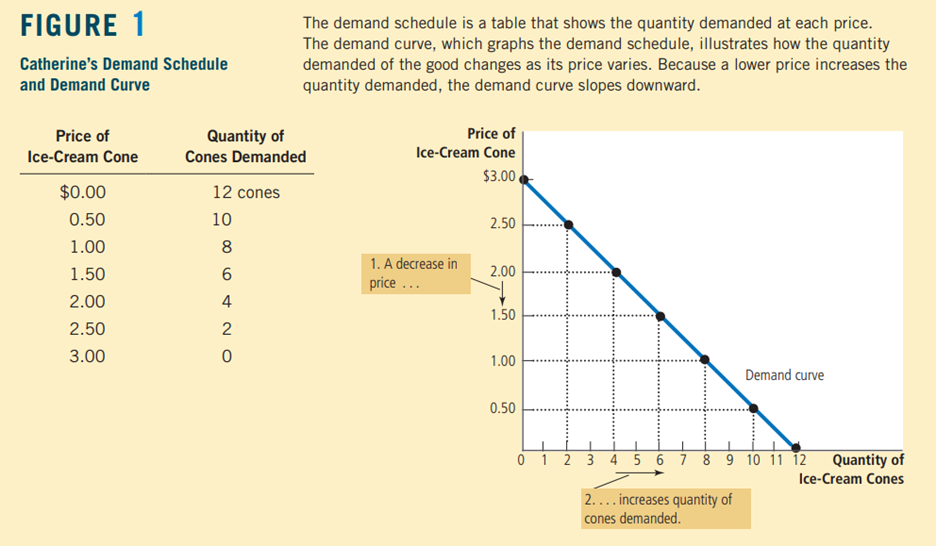
\includegraphics[width = 0.7\textwidth,keepaspectratio]{demand_curve.png}

    \begin{itemize}
    \item This example shows the demand curve for one individual. 
    \begin{itemize}
        \item The \textit{market demand} is the summation of demand curves across all individuals in a market.
    \end{itemize}
    \end{itemize}
\end{frame}

\begin{frame}{Types of Goods}
\begin{block}{Normal and Inferior goods:}
    \begin{itemize}
        \item \textbf{Normal goods}: demand increases when income increases
        \begin{itemize}
            \item Ex: travel
        \end{itemize}
        \item \textbf{Inferior goods:} demand decreases when income increases
        \begin{itemize}
            \item Ex: \textit{store brand} cereal
        \end{itemize}
    \end{itemize}
\end{block}

\begin{block}{Compliments and Substitutes:}
    \begin{itemize}
        \item \textbf{Complements}: two goods that go well together 
        \begin{itemize}
            \item Ex: peanut butter and jelly
        \end{itemize}
        \item \textbf{Substitutes:} two goods that fulfill the same purpose or class 
        \begin{itemize}
            \item Ex: coffee and tea
        \end{itemize}
    \end{itemize}
\end{block}
\end{frame}


\begin{frame}{Market demand}

\begin{block}{ Demand curves are not fixed in time; many things might cause a demand curve to change}
\begin{itemize}
\item Factors which cause movement along the demand curve: a \textit{change in price} of the good
\item Factors which shift the demand curve:
    \end{itemize}
\begin{center}
\begin{tabular}{ll}
\textbf{T: }& \textbf{T}astes/preferences \\
\textbf{R: }& prices of \textbf{R}elated goods \\
\textbf{I:} & \textbf{I}ncome of the buyers \\ 
\textbf{B:} & number of \textbf{B}uyers \\
\textbf{E: }& \textbf{E}xpectations of future prices \\
\end{tabular}
\end{center}
\end{block}
\medskip
   Q:  If goods A and B are complements, what will happen to demand for good B if the price of good A falls? What if they are substitutes?
   
\end{frame}


\begin{frame}{Example}
A few years ago Maryland passed a gas tax holiday, temporarily lowering the price of gasoline. Some critics said that lowering the tax would make people want to buy more gasoline and might end up actually \textit{increasing} the price.

    \begin{enumerate}
        \item Will the tax decrease cause the demand curve for gasoline to shift?
        \item What are some complements and what are some substitutes for gasoline?
        \item What are some factors that might cause the demand curve for gasoline to shift?
    \end{enumerate}

    Does it seem plausible that the tax increase could cause the price of gasoline to go up?

  \end{frame}

  \begin{frame}{Supply}
    \begin{itemize}
        \item \textit{Quantity supplied} is the amount sellers are willing and able to sell
        \item \textit{The law of supply:} as price increases, so does quantity supplied
\end{itemize}
 
 \begin{block}{Supply curves also are not fixed in time; many things might cause a supply curve to change} 
        \begin{itemize}
        \item Factors which cause movement along the supply curve: a change in price of the good
        \item \textit{Factors which shift the supple curve:} 
        \end{itemize}
    \begin{center}
\begin{tabular}{ll}
\textbf{P:} & \textbf{P}rices of inputs to production \\
\textbf{E:} & \textbf{E}xpectations about the future \\
\textbf{S:}& \textbf{S}ubsidies/taxes \\
\textbf{T:} & \textbf{T}echnology changes \\
\textbf{S:}& number of \textbf{S}ellers \\
\end{tabular}
\end{center}
\end{block}
        \end{frame}



 \begin{frame}{Equilibrium}
    Economists are generally interested in the point at which supply equals demand: \textit{equilibrium}
    
    \begin{block}{The equilibrium is characterized by two things:}
    \begin{itemize}
        \item Equilibrium \textbf{price} (\textit{market-clearing})
        \item Equilibrium \textbf{quantity}
    \end{itemize}
    \end{block}
    \medskip

    At this point:
    $$
    Q_D = Q_S
    $$
\end{frame}

\begin{frame}{Equilibrium}
    The actions of individuals in the market will naturally bring it into equilibrium: the \textit{law of supply and demand}.
    \begin{itemize}
        \item If there is excess supply there is a \textit{surplus}
        \item If there is excess demand there is a \textit{shortage}
    \end{itemize}
    \end{frame}
    

\begin{frame}{Market for gasoline}
    \begin{block}{Let's return to our question about gasoline, and run through some different scenarios...}
    What do the supply and demand curves for the market of gasoline look like, and what is the impact of the decrease in the gas tax?
\end{block}
    \begin{center}
        ** Does the tax cut cause a shift in demand or supply? **
    \end{center}
\end{frame}

\begin{frame}{Market for gasoline}
    \begin{block}{The tax cut caused the supply curve to shift to the right: }
        for any given price, sellers will supply a larger quantity at a lower price.
    \end{block}

    \medskip

    \begin{block}{Now suppose all cars experience a sudden increase in fuel efficiency: we can drive more miles with the same amount of gasoline}
        How does this affect supply or demand in our market for gasoline?
\end{block}
\end{frame}


\begin{frame}{Market for gasoline}
\begin{block}{ Increased fuel efficiency shifts our demand curve to the left} 
at any given price, we buy less gasoline than before, at a lower price.
\end{block}
    \medskip

   \begin{block}{Now think about the two changes together:}
   \begin{itemize}
       \item The gasoline tax is lowered
       \item Fuel efficiency increases
   \end{itemize}
    What is the net effect on the equilibrium quantity and price? Is it unambiguous?
    \end{block}


\end{frame}

\begin{frame}{Market for gasoline}
    The supply curve shifts to the right, and the demand curve shifts to the left:
    \begin{itemize}
        \item The equilibrium price is unambiguously lower
        \item The equilibrium quantity may increase or decrease; it depends on the magnitude of the two shifts!
    \end{itemize}
\medskip
\medskip
    Note that this falls right out of our supply and demand side analyses!
    \begin{itemize}
        \item In both cases, the price decreased
        \item With the tax cut, quantity increased, but with the fuel efficiency increase, quantity decreased
    \end{itemize}


\end{frame}

\begin{frame}{Market for Orioles tickets}
    In the last few years, the Orioles have gone from one of the worst teams in MLB to one of the best.

    \begin{enumerate}
        \item Draw the supply and demand curves for Orioles tickets.
        \item Does the supply curve look like it did in the gasoline market?
        \item Will the team's improved record effect supply or demand, and why?
        \item What will happen to equilibrium price and quantity?
    \end{enumerate}
\end{frame}

\begin{frame}{Market for Orioles tickets}
    \begin{itemize}
        \item Supply curve is vertical: why?
        \item A better team means more fans want to attend more games, shifting the demand curve to the right
        \item The equilibrium quantity is the same, but the price has increased
    \end{itemize}

    Is this a realistic way to think about the market for tickets?
\end{frame}

\begin{frame}{Market for Orioles tickets}
    Is this a realistic way to think about the ticket market?
    \begin{itemize}
        \item In some ways: we really do see ticket prices increasing, and the number of seats really is fixed
        \item In reality, not all seats are the same (different markets?) and not all seats get sold (there are fixed costs and frictions)
        \item Don't worry about any of this for now!
    \end{itemize}
\end{frame}

\end{document}